\section{Results}
\label{results}
\begin{figure}[htbp]
\begin{center}
\mbox{
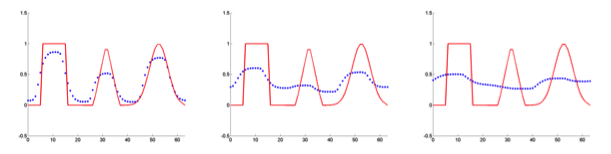
\includegraphics[width=0.31\textwidth]{First_Order_1.png}
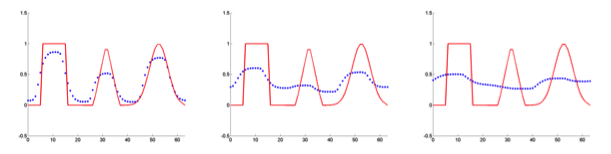
\includegraphics[width=0.31\textwidth]{First_Order_5.png}
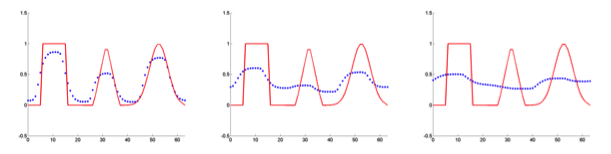
\includegraphics[width=0.31\textwidth]{First_Order_10.png}
} 
\mbox{  
\makebox[0.31\textwidth][c]{(a)}
\makebox[0.31\textwidth][c]{(b)}
\makebox[0.31\textwidth][c]{(c)}
}
\caption{Advection of a square wave, a triangular wave and an exponential wave over time with periodic boundary conditions after (a) 1 pass through the domain, (b) 5 passes through the domain and (c) 10 passes through the domain using a central differencing first order method.}
\label{First_Order}
\end{center}
\end{figure}

\begin{figure}[htbp]
\begin{center}
\mbox{
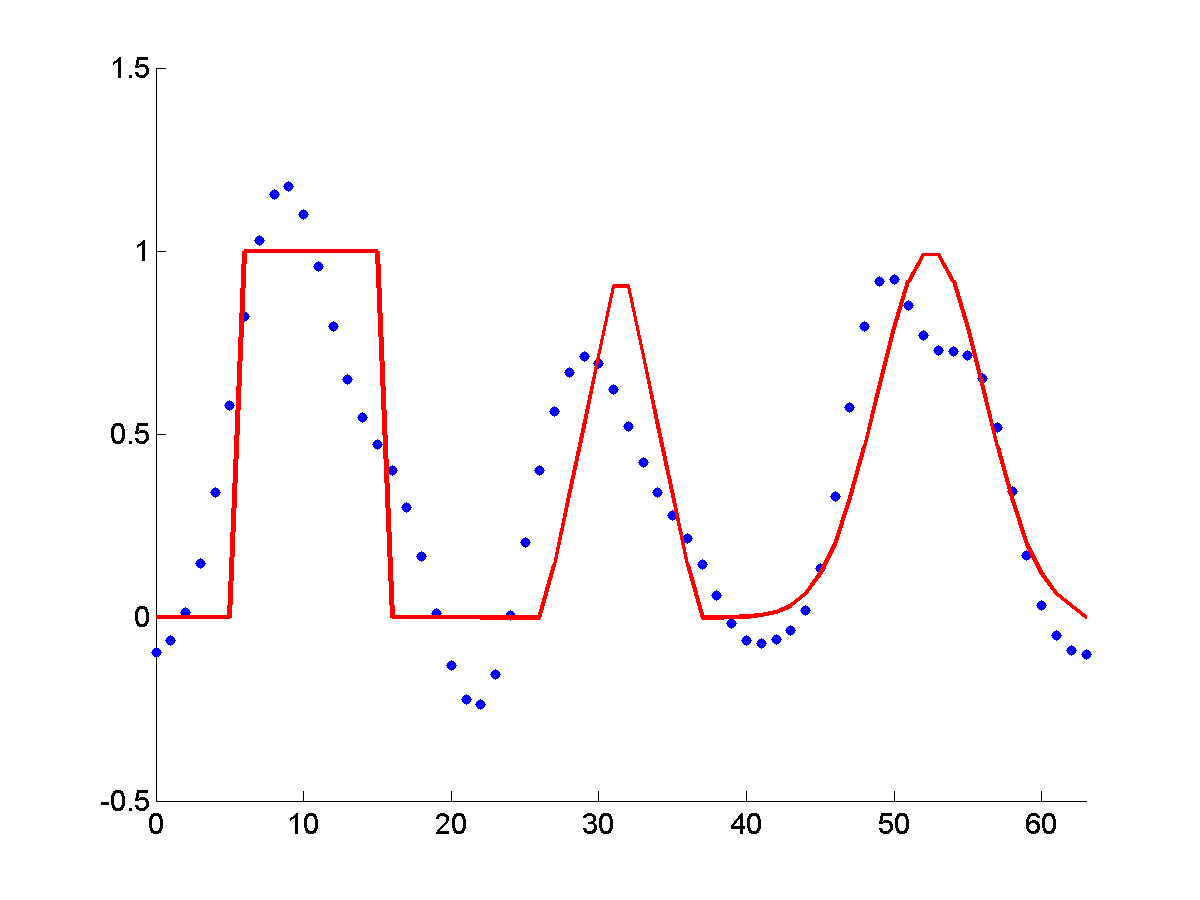
\includegraphics[width=0.31\textwidth]{Lax-noTVD_1.png}
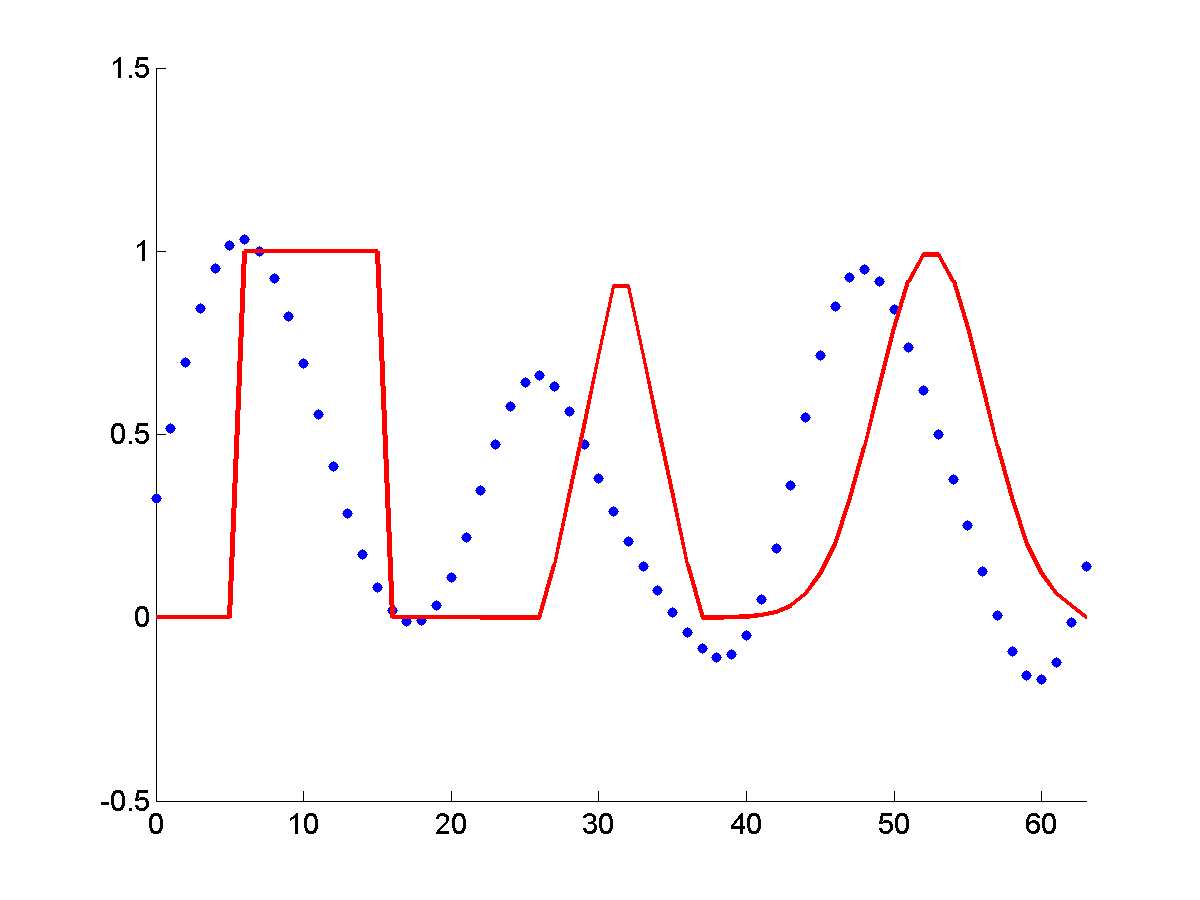
\includegraphics[width=0.31\textwidth]{Lax-noTVD_5.png}
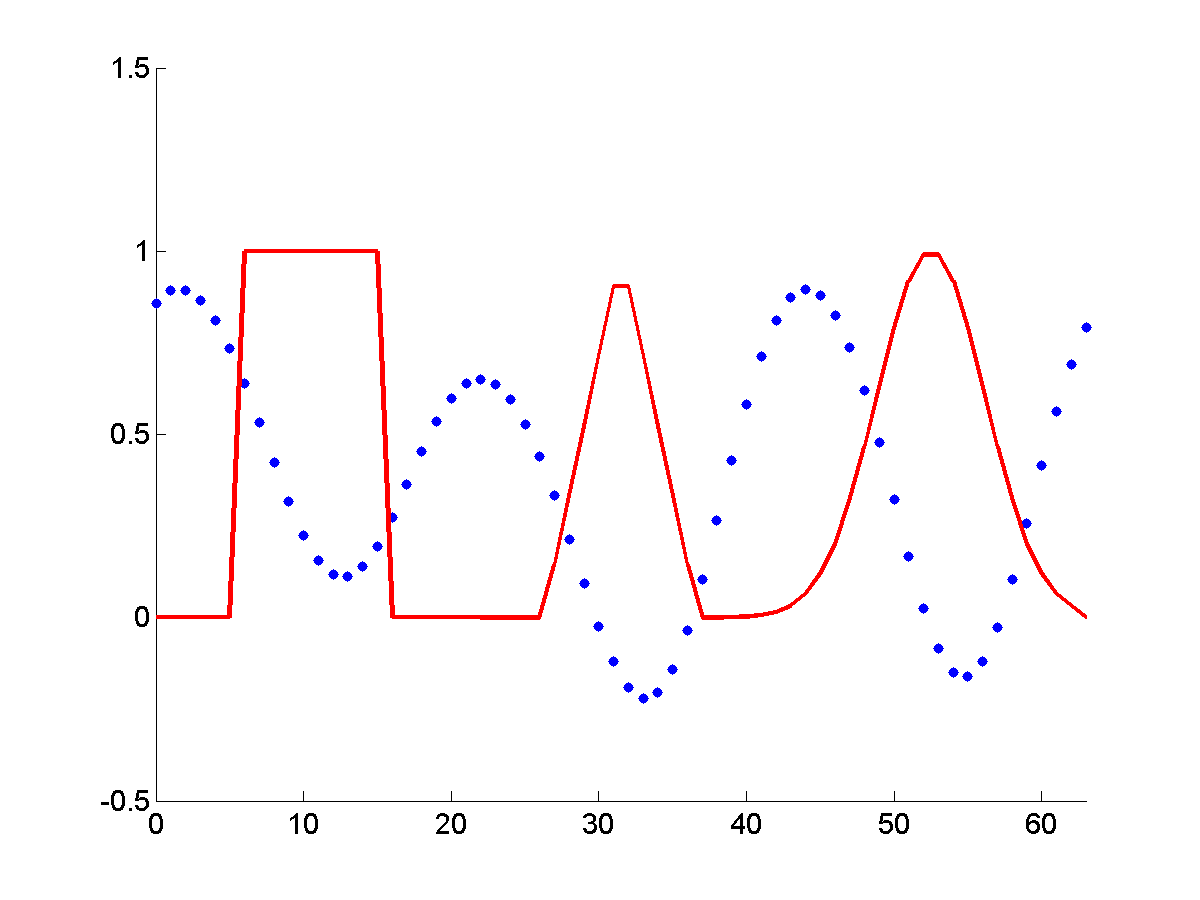
\includegraphics[width=0.31\textwidth]{Lax-noTVD_10.png}
} 
\mbox{  
\makebox[0.31\textwidth][c]{(a)}
\makebox[0.31\textwidth][c]{(b)}
\makebox[0.31\textwidth][c]{(c)}
}
\caption{Same caption as Figure \ref{First_Order} except that a Lax-Wendroff method without any slope limiters was used to advect the waves.}
\label{Lax-noTVD}
\end{center}
\end{figure}

\begin{figure}[htbp]
\begin{center}
\mbox{
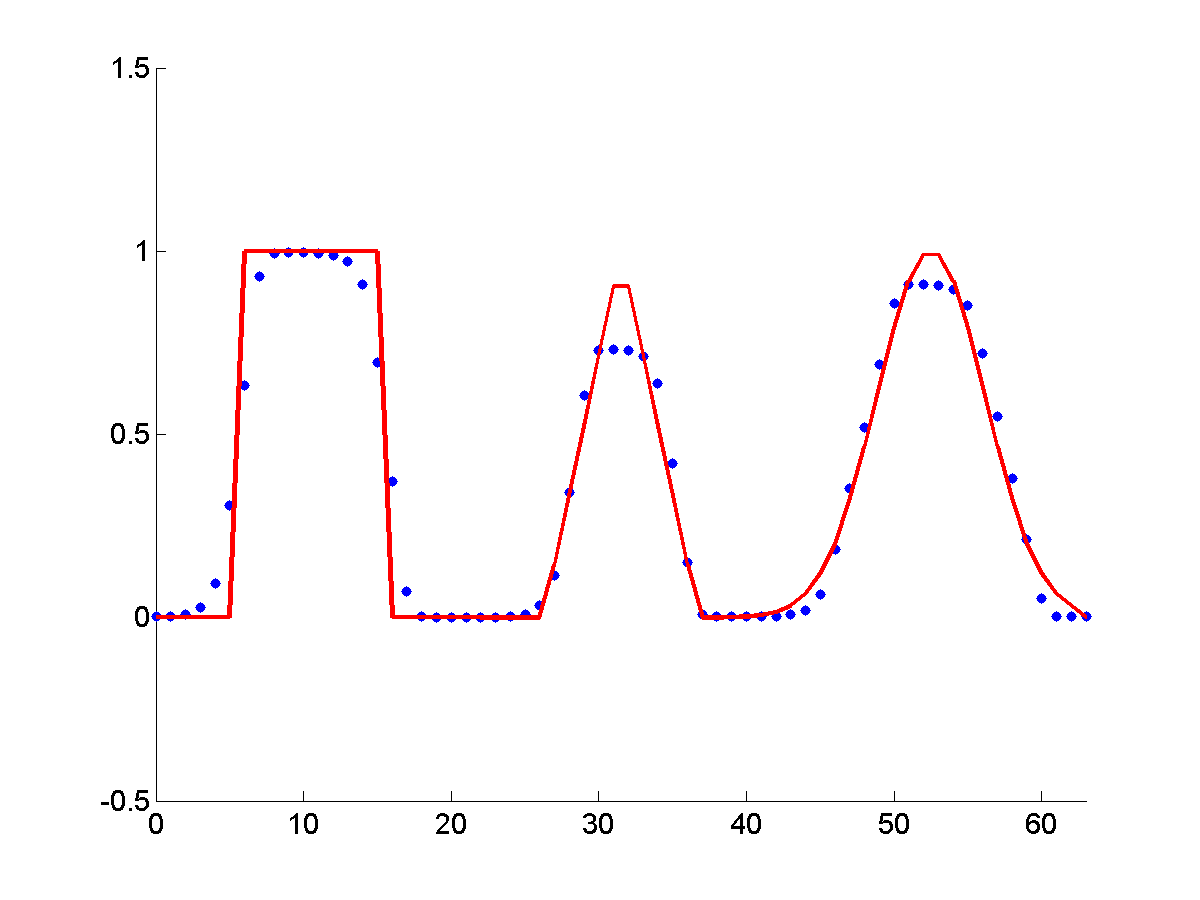
\includegraphics[width=0.31\textwidth]{Lax-wTVD_1.png}
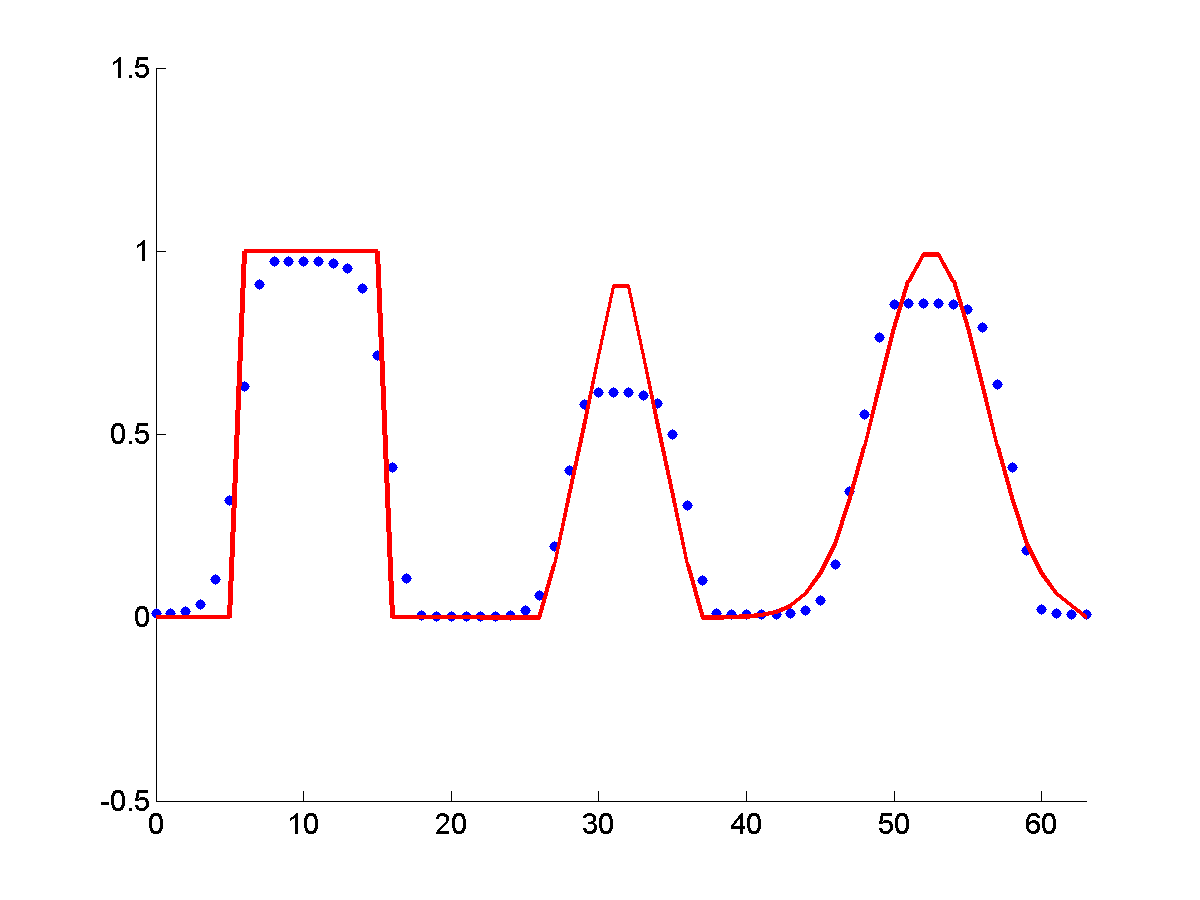
\includegraphics[width=0.31\textwidth]{Lax-wTVD_5.png}
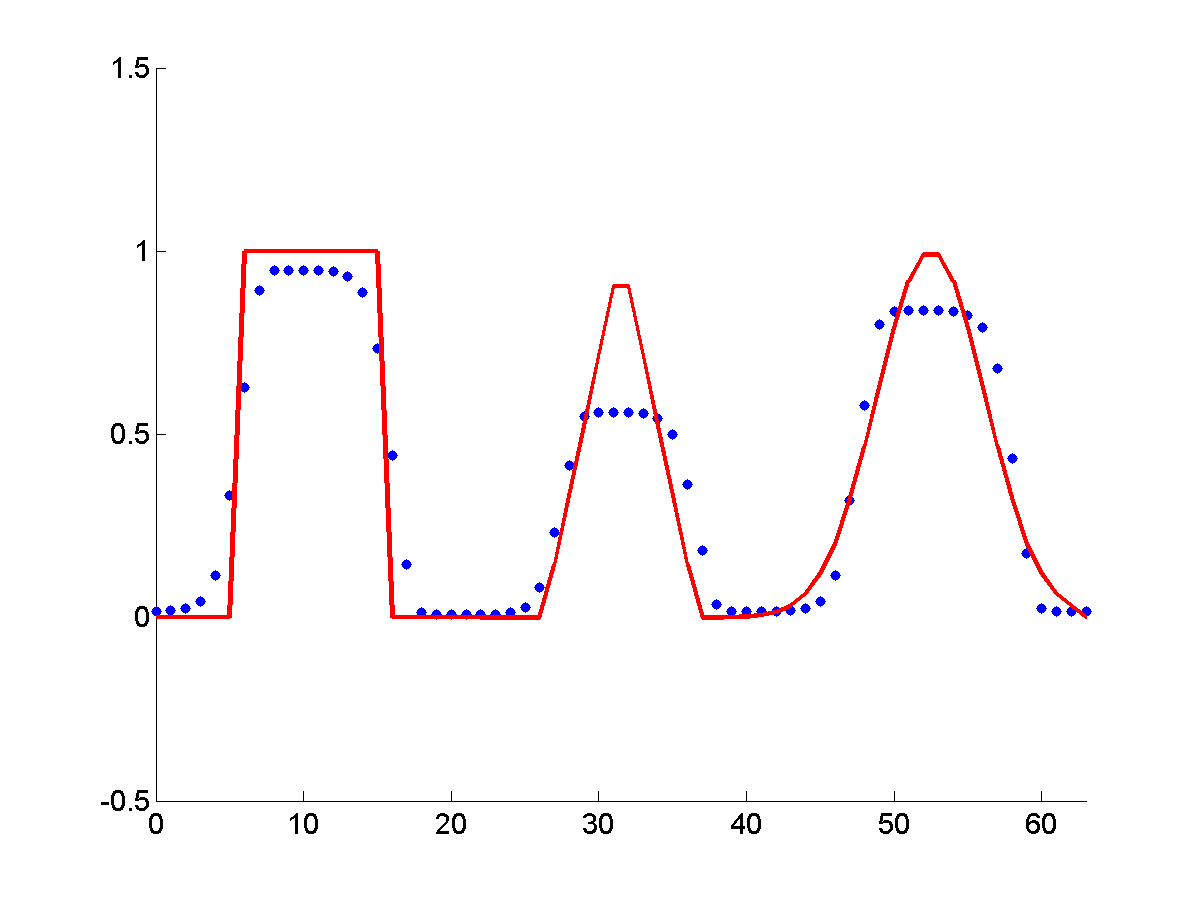
\includegraphics[width=0.31\textwidth]{Lax-wTVD_10.png}
} 
\mbox{  
\makebox[0.31\textwidth][c]{(a)}
\makebox[0.31\textwidth][c]{(b)}
\makebox[0.31\textwidth][c]{(c)}
}
\caption{Same caption as Figure \ref{First_Order} except that a Superbee Limiter was used along with the Lax-Wendroff method to advect the waves.}
\label{Lax-wTVD}
\end{center}
\end{figure}

\begin{figure}[htbp]
\begin{center}
\mbox{
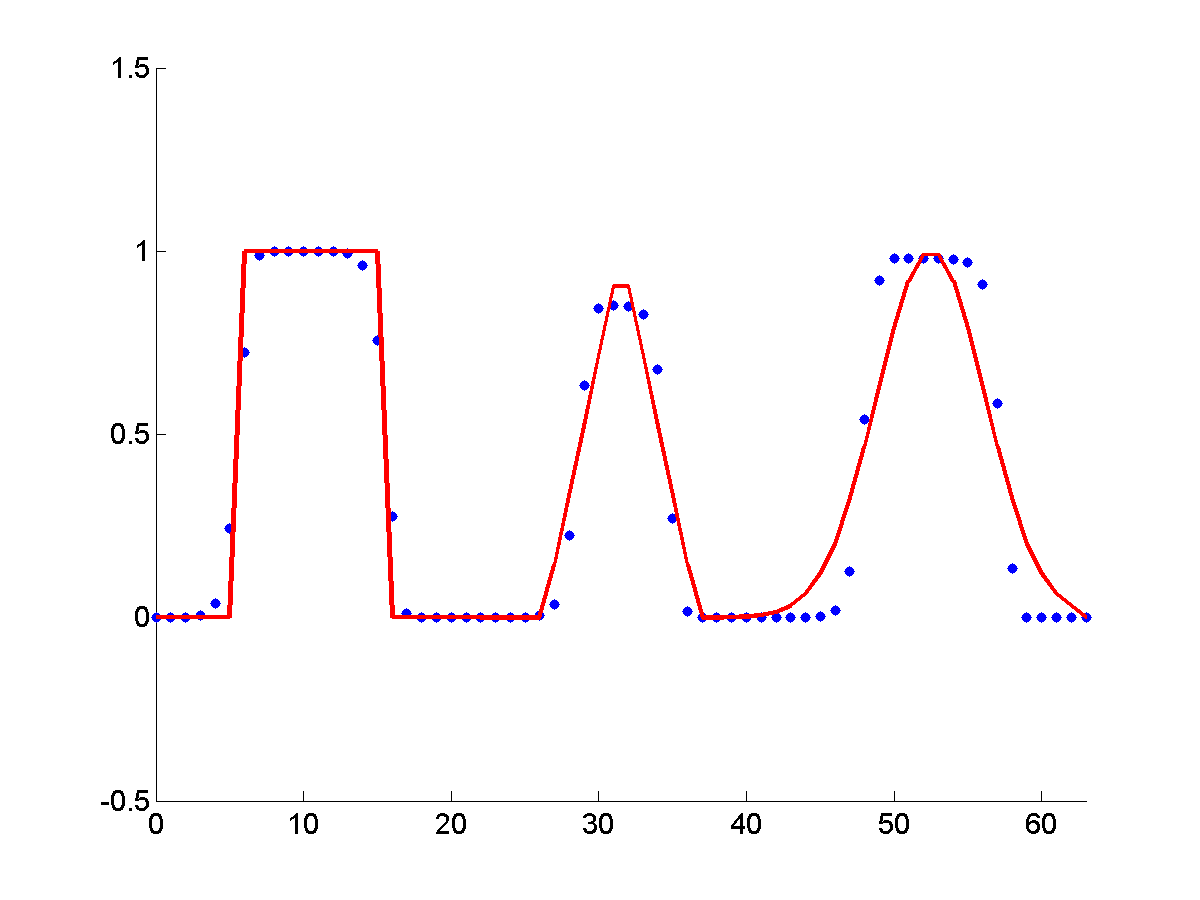
\includegraphics[width=0.31\textwidth]{MUSCL_1.png}
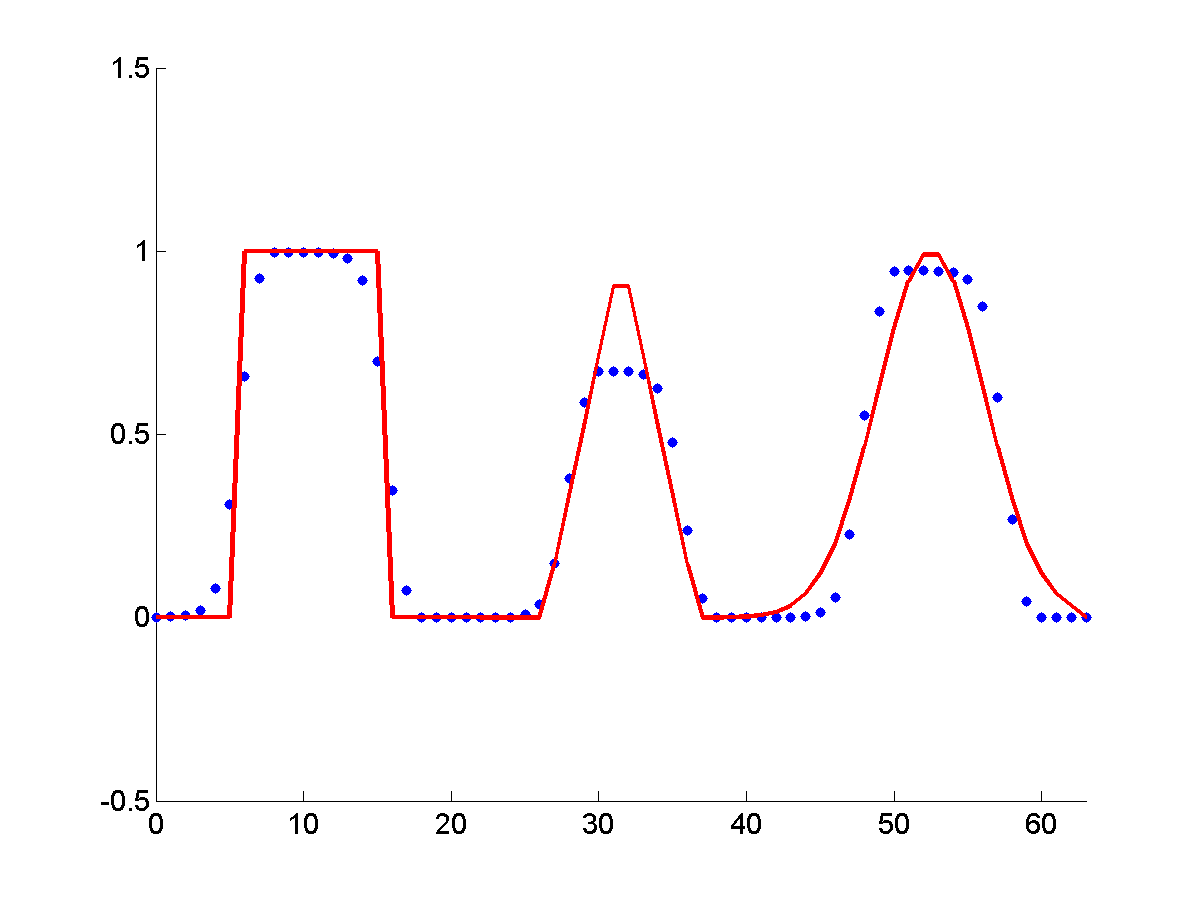
\includegraphics[width=0.31\textwidth]{MUSCL_5.png}
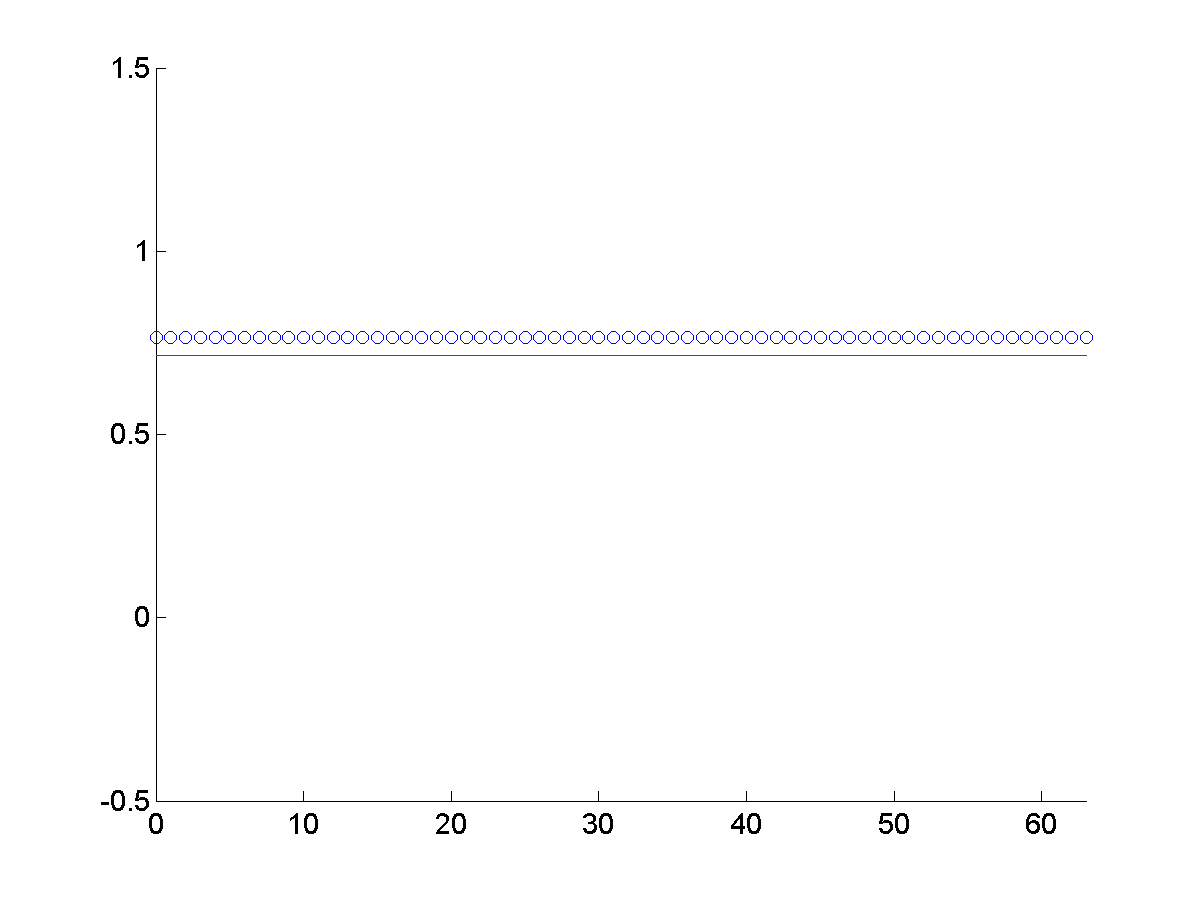
\includegraphics[width=0.31\textwidth]{MUSCL_10.png}
} 
\mbox{  
\makebox[0.31\textwidth][c]{(a)}
\makebox[0.31\textwidth][c]{(b)}
\makebox[0.31\textwidth][c]{(c)}
}
\caption{Same caption as Figure \ref{First_Order} except that a MUSCL with an ACM were used advect the waves.}
\label{fig:MUSCL}
\end{center}
\end{figure}

\begin{figure}[htbp]
\begin{center}
\mbox{
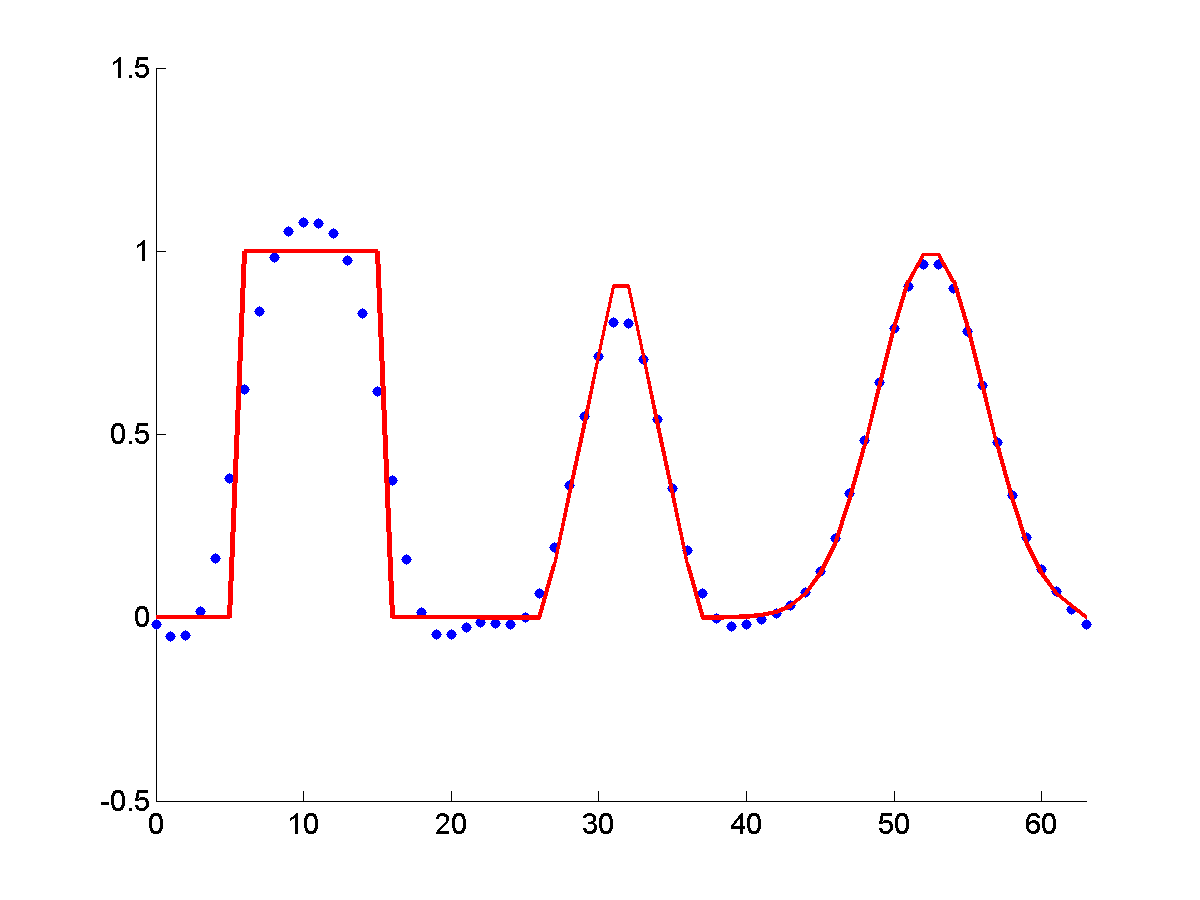
\includegraphics[width=0.31\textwidth]{SUPG_1.png}
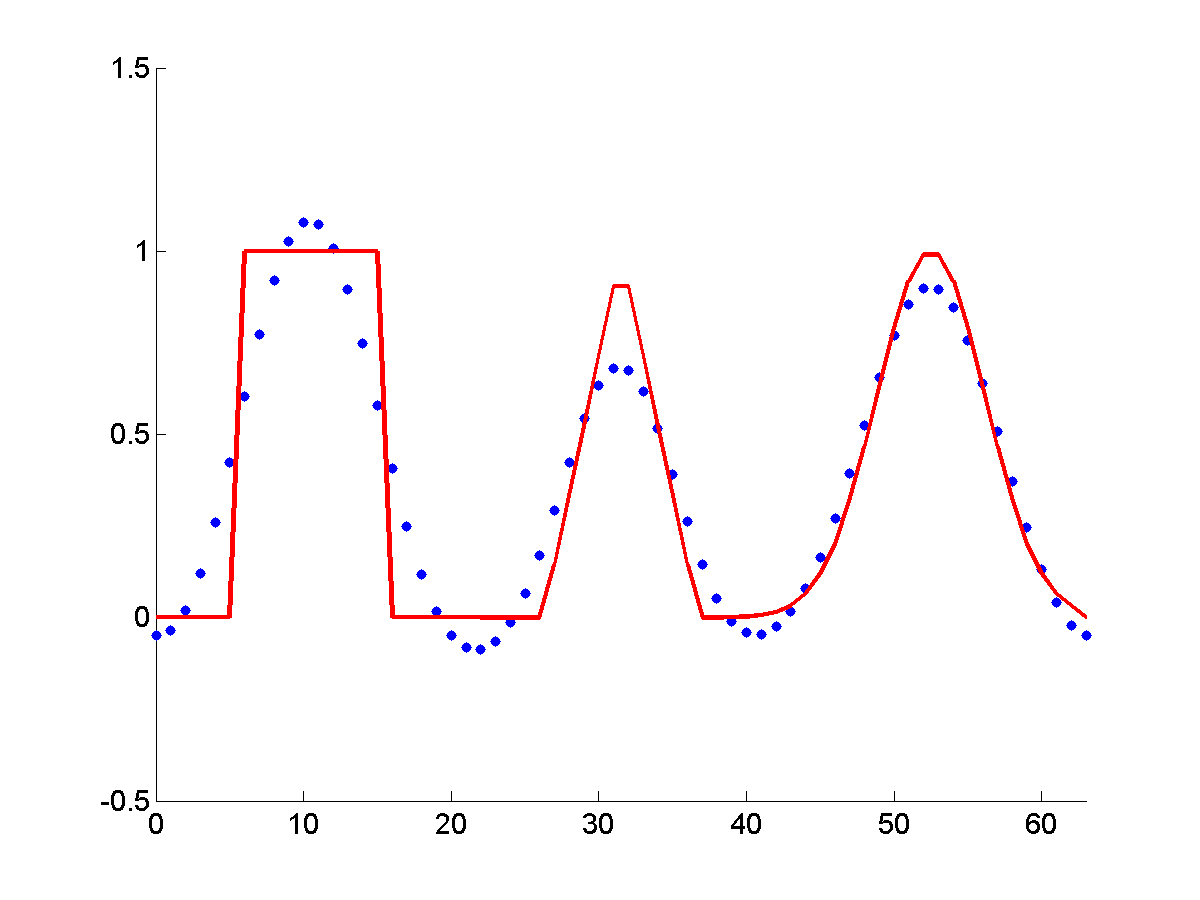
\includegraphics[width=0.31\textwidth]{SUPG_5.png}
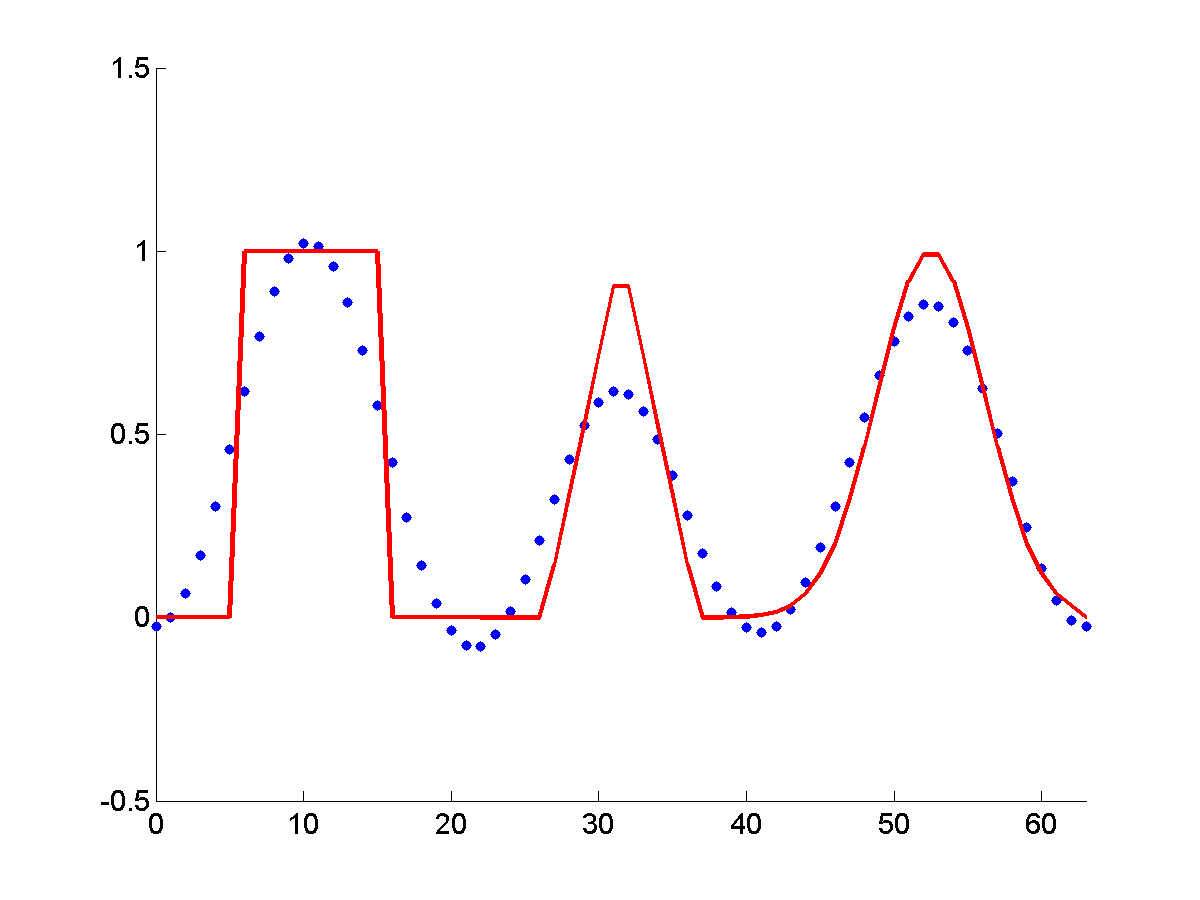
\includegraphics[width=0.31\textwidth]{SUPG_10.png}
} 
\mbox{  
\makebox[0.31\textwidth][c]{(a)}
\makebox[0.31\textwidth][c]{(b)}
\makebox[0.31\textwidth][c]{(c)}
}
\caption{Same caption as Figure \ref{First_Order} except that SUPG was used to advect the waves.}
\label{fig:SUPG}
\end{center}
\end{figure}

\begin{figure}[htbp]
\begin{center}
\mbox{
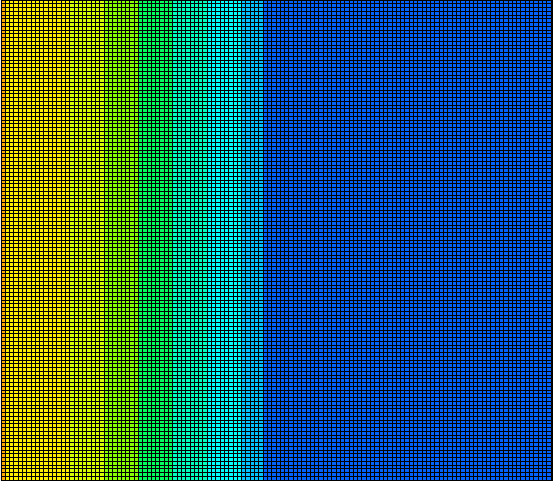
\includegraphics[width=0.31\textwidth]{H_1.png}
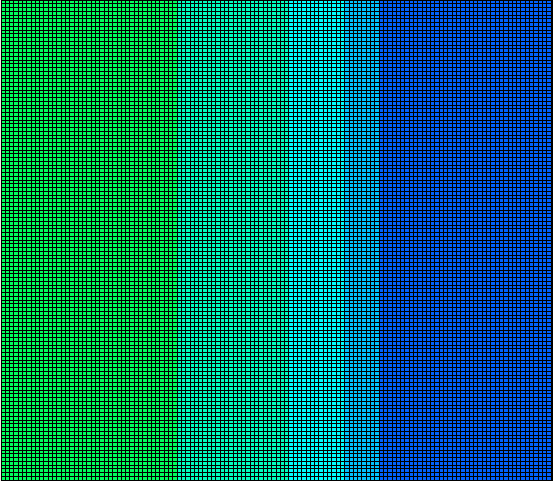
\includegraphics[width=0.31\textwidth]{H_10.png}
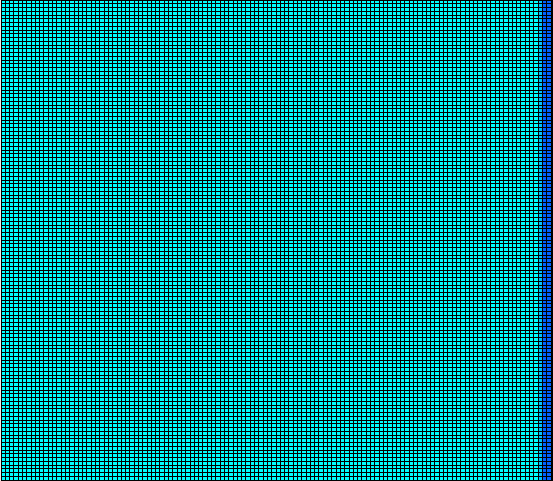
\includegraphics[width=0.31\textwidth]{H_20.png}
} 
\caption{Evolution of the height of a wave over time using the GPU enabled wave code.}
\label{fig:H}
\end{center}
\end{figure}

\begin{figure}[htbp]
\begin{center}
\mbox{
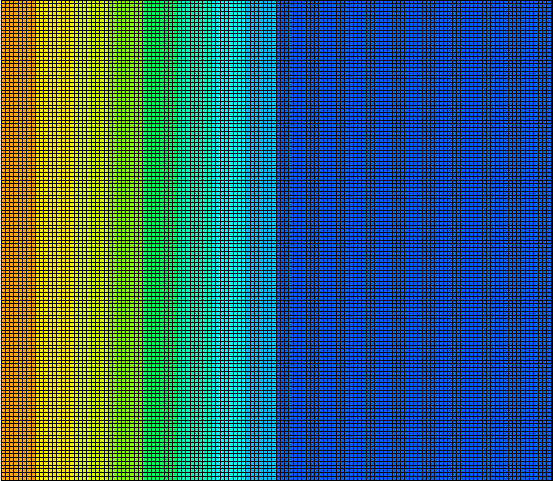
\includegraphics[width=0.31\textwidth]{phi_1.png}
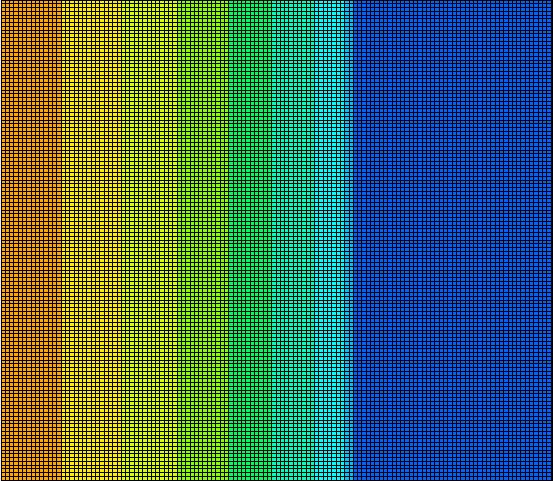
\includegraphics[width=0.31\textwidth]{phi_10.png}
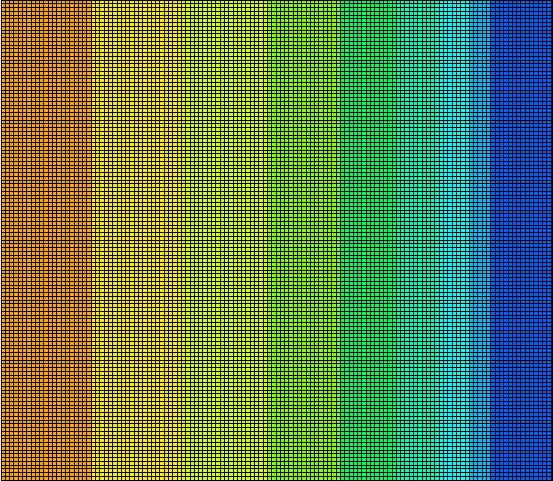
\includegraphics[width=0.31\textwidth]{phi_20.png}
} 
\caption{Evolution of the concentration of a dye over time using the GPU enabled wave code.}
\label{fig:H}
\end{center}
\end{figure}